\documentclass[conference]{sty/IEEEtran}
\usepackage{times}
\usepackage{wrapfig}
\usepackage{tweaklist}
\usepackage{xspace}
\usepackage{graphicx}
\usepackage{subfigure}
\usepackage{tabularx}
\usepackage{amsmath}
\usepackage{amssymb}
\usepackage{url}
\usepackage{bm}
\usepackage{color}
\usepackage{colortbl}

\def\cH{\mathcal{H}}
\def\cL{\mathcal{L}}
\def\cP{\mathcal{P}}
\def\cO{\mathcal{O}}
\def\mP{{\mathsf P}}
\def\mh{{\mathsf h}}
\def\mo{{\mathsf o}}
\def\mv{{\mathsf v}}
\def\mn{{\mathsf n}}
\def\vcb{{\boldsymbol{c}}}
\def\vpb{{\boldsymbol{p}}}
\def\vqb{{\boldsymbol{q}}}
\def\vnb{{\boldsymbol{n}}}
\def\vlb{{\boldsymbol{l}}}
\def\mr{{\mathsf r}}


% numbers option provides compact numerical references in the text.
\usepackage[numbers]{natbib}
\usepackage{multicol}
\usepackage[bookmarks=true]{hyperref}

% \pdfinfo{
%    /Author (Homer Simpson)
%    /Title  (Robots: Our new overlords)
%    /CreationDate (D:20101201120000)
%    /Subject (Robots)
%    /Keywords (Robots;Overlords)
% }

\begin{document}

% paper title
%\title{Classification of Objects of Daily Use Using Combined Color CHLAC and Global Radius-based Surface Descriptors}
%\title{Multidimensional Descriptor for Classification of Objects of Daily Use}
\title{Voxelized Shape and Color Histograms for RGB-D}

% You will get a Paper-ID when submitting a pdf file to the conference system
\author{Paper-ID [110]}

% \author{\authorblockN{Asako Kanezaki, Tatsuya Harada}
% \authorblockA{
% Graduate School of Information \\ Science and Technology,\\
% University of Tokyo \\ %7-3-1 Hongo Bunkyo-ku, Tokyo Japan \\
% Email: \{kanezaki, harada\}@isi.imi.i.u-tokyo.ac.jp}
% \and
% \authorblockN{Dejan Pangercic, Zoltan-Csaba Marton, Michael Beetz}
% \authorblockA{
% Intelligent Autonomous Systems Group,\\ TU Munich \\
% Email: \{pangercic, marton, beetz\}@cs.tum.edu}}

\newcommand{\todo}[1]{\textbf{\textcolor{red}{TODO: #1}}}
\maketitle

\begin{abstract}
The greatest bottleneck momentarily in the area of mobile manipulation is robust perception.
In this paper we contribute to the solving of this problem of efficiency and accuracy
by proposing a novel feature called Voxelized Shape and Color Histograms 
(VOSCH) that is capable of capturing both the geometric and visual appearance
properties of common objects of daily use. We showcase the
feature's applicability for the purpose of classification of objects in cluttered scenes with occlusions,
and evaluate two classification approaches.
For the experiments we make use of a new RGB-D device called Kinect, and achieve recognition
rates higher than 90\% for a set of 63 objects.
\end{abstract}

\IEEEpeerreviewmaketitle

\section{Introduction}
One of the great challenges in autonomous mobile robot manipulation is scaling
technology to realistic tasks, in real-world environments under realistic
conditions. This means that an autonomous household robot must act on many
different objects of daily use, handle them in typical situations such as
opening a fridge to get the milk or when performing challenging everyday tasks
such as setting the table or preparing a meal.

%\todo{Provide the definition of descriptor vs detector vs feature}\\
Descriptor-based object recognition has proved over last years to be very successful.
SIFT~\cite{lowe04distinctive}, SURF~\cite{surf} and others can
detect, localize and recognize many types of textured objects efficiently, reliably
and under varying lighting conditions. Likewise descriptors have been developed 
for perceiving objects based on their shapes (e.g. circles, cylinders, spheres and hybrid variants).
Normal Aligned Radial Features (NARF)\cite{steder10irosws} for range images, 
and several versions of Point Feature  Histograms (PFH, FPFH)~\cite{Rusu09ICRA} and 
Viewpoint Feature Histograms (VFH)~\cite{vfh} for unordered fully-3D point clouds are just 
to name a few. While these descriptors were successful too, they are still limited because they
typically work only in restricted feature spaces. So, in order to have perception system
based on SIFT features, one needs to restrict search space to objects that are detected by
texture, if we apply 3D feature the objects must be distinctive with respect to their shapes. 
If we really want to install a perception system for autonomous robots we need to aim 
at one that can perceive all objects, that is textured, texture-less, different shapes, etc.
While it seems feasible that we can simply develop perception routines by combining
various descriptors~\cite{stueckler10combining, GRSD10Humanoids}, the more promising idea 
is to develop descriptors that work in multiple feature spaces. The reason for this is 
that objects might be easily discriminated in combined feature space whereas it is impossible 
to discriminate them in individual spaces as depicted in Figure~\ref{fig:grsd_cchlac}.
In this paper we propose a novel descriptor which builds off the idea of the previously 
published Global Radius-based Surface Descriptor (GRSD~\cite{GRSD10Humanoids}) and 
Color Cubic Higher-order Local Auto-Correlation descriptor (ColorCHLAC~\cite{kanezaki2010tvc}), 
and which we call Voxelized Shape and Color Histograms (VOSCH).

\begin{figure}[htb!]
  \begin{center}
    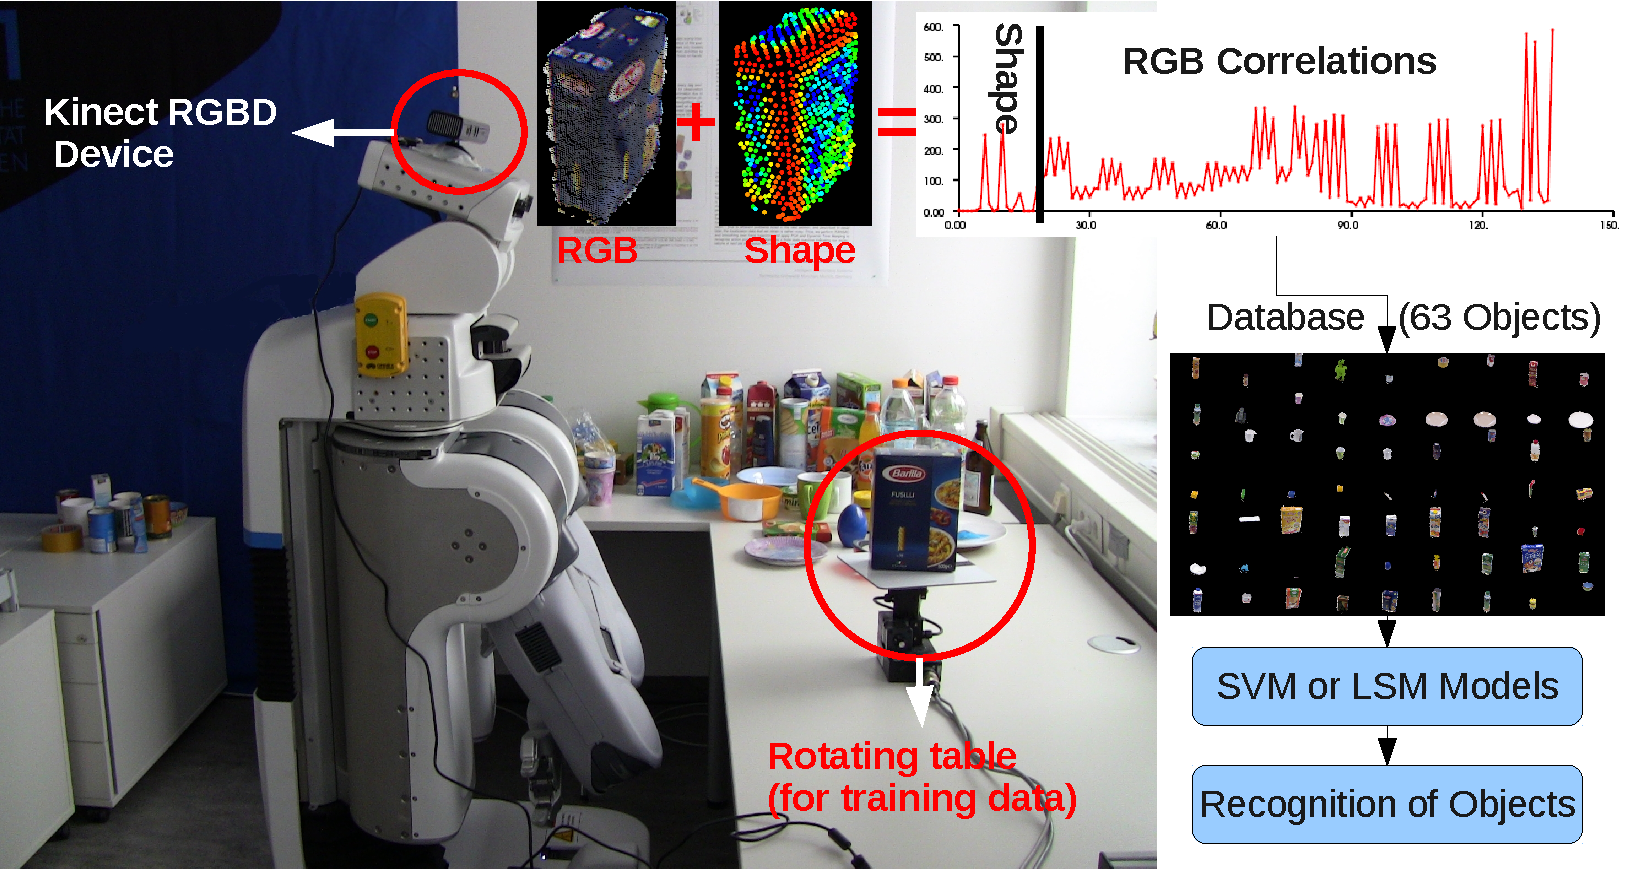
\includegraphics[width=.99\columnwidth]{figures/firstpage/firstpage.pdf}
    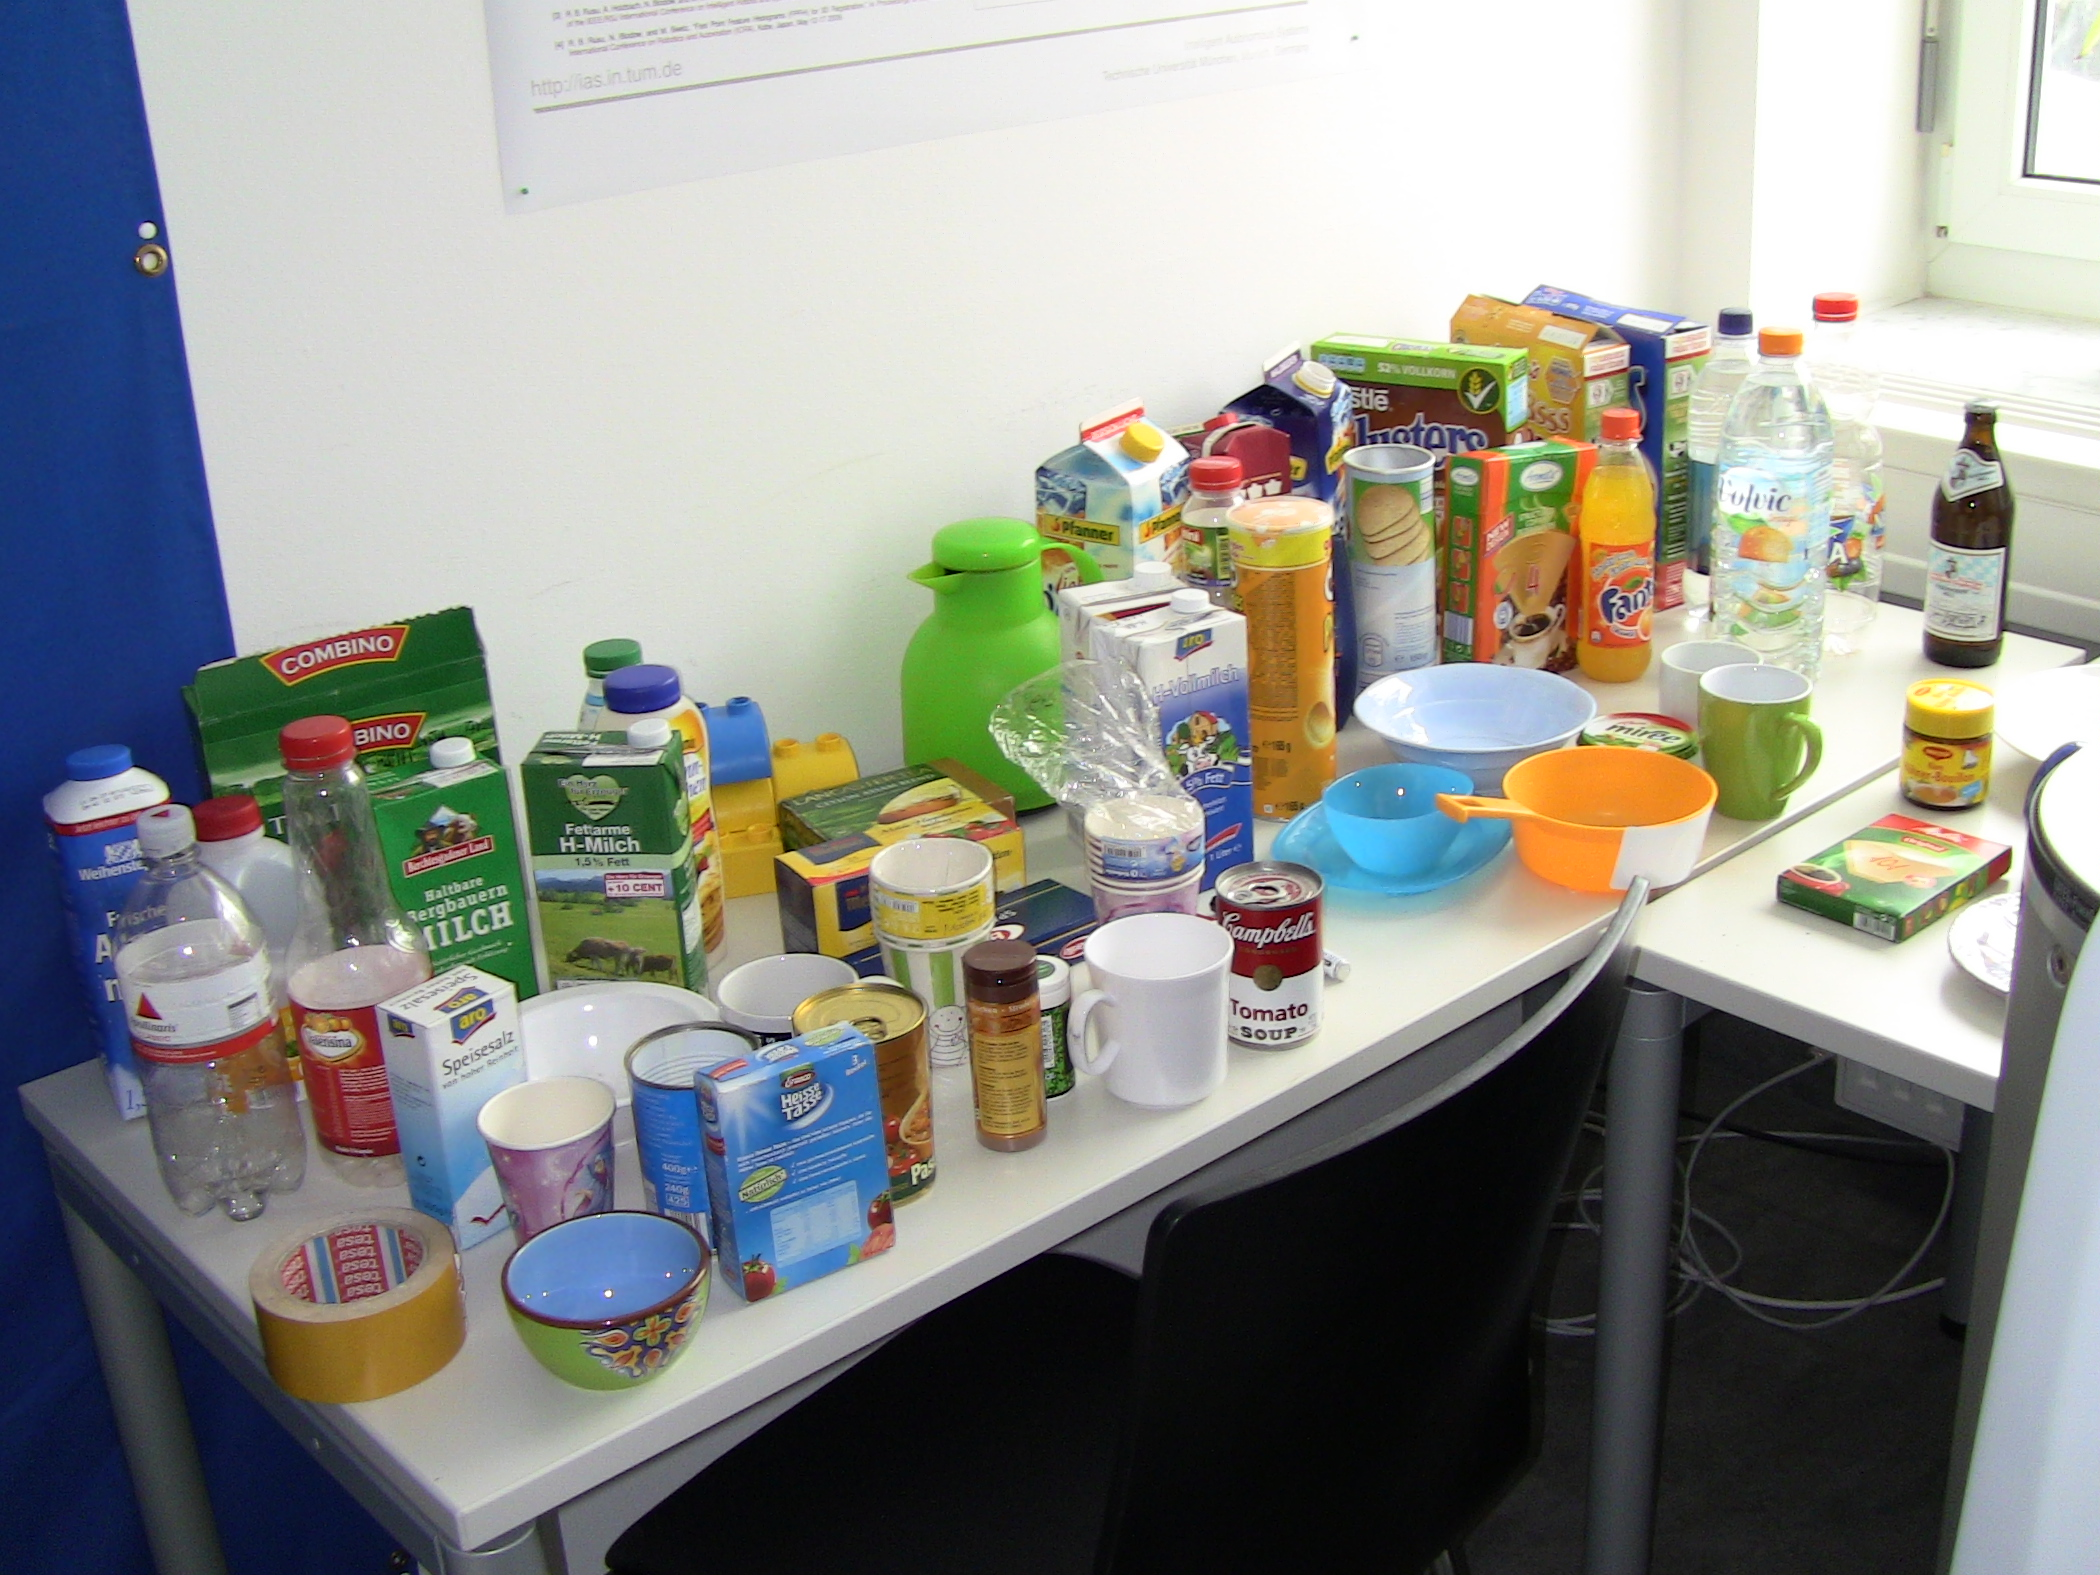
\includegraphics[width=.99\columnwidth]{figures/objects/objects.jpg}
    \caption{Top: Autonomous service robot equipped with a Kinect sensor
    acquiring training data of the objects shown in the bottom image. For 
  every view of the object VOSCH descriptor was estimated and a database
of 63 objects was generated. Object detection pipeline with Support Vector
Machine or Linear Subspace Method classifiers was then use to detect objects
in natural scenes.}
    \label{fig:robot}
  \end{center}
\end{figure}

% \subsection{What}
% In this paper, we address the problem of localization and recognition of
% objects of daily use in households. To this effect, we employ a multidimensional
% feature descriptor that captures both the geometrical and visual appearance
% properties of the objects.

The strength of the descriptor lies in its ability to consider geometric and
visual features in a unified manner to facilitate object classification. The two
underlying features (GRSD, ColorCHLAC) have been carefully selected because of their similar structures
and the way they are computed from voxelized 3D data. Their combination is
not a mere concatenation of two different features, but their computation is
performed in a single step because of the common underlying algorithmic
properties. Both features %though independently developed, 
count relations between neighboring voxels, capturing geometric surface type and texture
transitions at the same time.

Further contributions of work presented herein include the ability to deal with
cluttered scenes while eliminating the requirement for region of interest
selection (e.g. horizontal supporting structures) and spatially separable object
clusters. This has been achieved using a moving-bounding-box-based approach, and
a sub-space-matching-based classification scheme (Section
\ref{sec:recognition}). The resulting approach performs at 2 frames per second
while taking into account an object database of 63 different objects
(see Figure~\ref{fig:robot}).

% \subsection{Why}
% In the past, strong features have been proposed in perception for personal robots,
% both working on 2D and 3D data. Prominent examples include
% SIFT~\cite{lowe04distinctive} and SURF~\cite{surf} for camera images, Normal Aligned Radial
% Features (NARF)\cite{steder10irosws} for range images, and several versions of Point Feature
% Histograms (PFH, FPFH)~\cite{Rusu09ICRA} and Viewpoint Feature Histograms
% (VFH)~\cite{vfh} for unordered fully-3D point clouds.
% \todo{Nico proof-read till here}


% Yet it seems that there is none that can capture
% all important and obvious properties (such as geometry and color are)
Lastly, our descriptor can be out-of-the box applied on the data coming out of the 
new sensing technologies such as Kinect device and lays the foundation stone for a
multitude of applications such as later presented recognition of a priori learned object models
(Section~\ref{sec:recognition}). VOSCH also enables equipping of service robots 
(such as the robot shown in top part of Figure~\ref{fig:robot}) with the 
capabilities to acquire additional object models which furthermore opens ways 
for manipulation tasks in realistic environments under realistic conditions.

\begin{figure}[htb!]
  \begin{center}
    \includegraphics[width=.48\columnwidth]{figures/colorCHLAC/artificial/purple.png}
    \includegraphics[width=.48\columnwidth]{figures/colorCHLAC/artificial/torus.png}
    \caption{Examples of \todo{scaled} VOSCH histograms.
Left: different categories of objects (top-down: cone, cube, cylinder, plane, sphere, torus, dice) 
result in having different first 20 bins of the respective histogram.
Right: different colors of the same category of an object torus have different 137 right-most bins of the histogram}
    \label{fig:grsd_cchlac}
  \end{center}
\end{figure}

The remainder of the paper is built as following. After the overview of the related
work in Section~\ref{sec:rl} we present the major system components in Section~\ref{sec:overview}
which is followed by Section~\ref{sec:features} that elaborates on the construction of the
VOSCH descriptor. In Section~\ref{sec:classification} we present the usage of this descriptor
for the classification of objects using two classification methods which we
then elaborately test and present in Section~\ref{sec:results}. In Section~\ref{sec:conclusion}
we conclude and give the future outlook.



\section{Related Work}
\label{sec:rl}
%\item Color CHLAC (Asako)~\cite{kanezaki2010icra}\cite{kanezaki2010tvc}
% \item textured-spin images~\cite{Johnson_spin_images}
% \item A sparse texture representation using local affine
% regions~\cite{Lazebnik05asparse}
% \item sift-keypoint
% \url{http://www.ros.org/doc/api/pcl/html/sift__keypoint_8h_source.html}
Expressiveness and efficiency of the descriptor are both crucially important for
a real-time object recognition system.  Though there is a trade-off between
these two abilities, it will dramatically improve both of them to select a
proper matching method taking advantage of the characteristics of the
descriptor. In the recent decade a corpus of powerful 2D and 3D descriptors for
recognizing real objects have been developed, however, few of them take into
account the compatibility with the matching method used with them.

SIFT~\cite{lowe04distinctive} descriptor, one of the most well-known 2D
descriptors for object recognition, makes use of detected keypoints in
scenes and compares them with those of reference objects to identify the
objects currently observed. A combination of the visual appearance
descriptor and 2D shape is presented by Bosch et al. in~\cite{Bosch07shape}
where they use random forests to achieve around 80\% of classification 
accuracy. Half-way through to 3D domain an effective descriptor
NARF~\cite{steder10irosws}, which detects salient points in range images of
real environments, has recently been developed.  Despite of their dominant
repeatability in point-to-point matching, there still remains difficulty in
cluster-to-cluster matching, which is necessary for identifying each cluster
candidates  in environments as objects. This also causes computational expensiveness
especially when the target object database is large. In 3D domain a recently 
developed VFH~\cite{vfh} descriptor was presented as an extension 
of~\cite{Rusu09ICRA}. The feature's discriminative power is boosted up
by an inclusion of viewpoint which on the other side however represents
the deficiency in that it becomes orientation variant. 

There are few approaches that use both geometry and color descriptors to
represent 3D shapes~\cite{park2006}, however, to properly balance these two
different properties is difficult.  Caputo and Dorko~\cite{caputo2002} learned
respective kernels for shape and color representations and combined them for
recognition object, while Huang and Hilton~\cite{huang2009} balanced them by
normalizing bins of shape-color histograms.  Alternative solution for combining
geometry and color information at a proper balance is to extract descriptors
represented by patterns of shape-and-color co-occurrence.  For example, Textured
spin-image~\cite{cortelazzo2006} splits well-known
spin-image~\cite{Johnson_spin_images} descriptors into several layer
corresponding to a given level of luminance. Color-CHLAC~\cite{kanezaki2010icra} 
splits CHLAC~\cite{kobayashi2004} descriptor, which is a histogram of 14 patterns 
depending on relative position of neighboring voxels, into RGB channels and correlation 
space of these channels.  In \cite{kanezaki2010icra} Color-CHLAC descriptor is used as local
descriptors in the training process and as a global descriptor describing each
object cluster in the recognition process, taking advantage of the combination
of Linear Subspace Method (LSM)~\cite{watanabe1973} and the descriptor's additive property, 
which means a global descriptor for an object cluster is computed by summing up local descriptors of its sub-parts.

\section{System Overview}
\label{sec:overview}
Systematically the idea of the whole work presented herein is depicted in 
Figure~\ref{fig:robot}. We first acquired the training data of 63 objects
of daily use using RGBD Kinect sensor. Then we estimated VOSCH descriptor 
for every object view and generated training models using Support Vector
Machine or Linear Subspace Method classifiers. The models were used
in the evaluation part for cross-validation checks and detection of 
objects in natural scenes.

Since the focus of the paper is on three parts, i.e. i)VOSCH descriptor
construction, ii)database assembly and training of object models and iii)testing,
we solved each of them individually. In the first case we had to unify underlying
structures such that the ColorCHLAC became rotation invariant and GRSD 
additive~\cite{kanezaki2010tvc}. We thus obtained a descriptor histogram with 
137 bins representing the transitions between its different dimensions.
In the second case, we assembled a large database of
object models (Figure~\ref{fig:robot} bottom), by creating a rotating
table using a DP PTU47 pan-tilt unit that is controlled by the robot over the
network. Objects placed on this rotating table were scanned at a given
angle-step ($15^\circ$) and dumped to the disk. The resultant database of
object models was then used to classify objects found in
natural table setting scenes while performing manipulation
tasks. For this third case we also performed a test on objects that were
segmented in the euclidean sense. 

Our approach is realized as part of the Robot Operating System
(ROS)\footnote{\url{http://www.ros.org}} open source initiative, and makes
use of modular and robust components that can be reused on other robotic
systems different than ours.

\subsection{Performance and Novelty}
Our approach takes 404 seconds for the training of 63 objects and 3.15 seconds
for the classification using Support Vector Machine classifier. Moving-bounding-box-based
recognition of objects in e.g. cluttered scenes takes 0.5 second as detailed
in Section~\ref{sec:recognition}.

The main novel contributions of this paper are the following:
\begin{itemize}
\item novel, multidimensional descriptor VOSCH that accounts for
geometrical as well as visual appearance  properties of objects in question
\item comparison of classification results for two established classification
frameworks; Linear Subspace Method~\cite{watanabe1973} and Support Vector Machine~\cite{svm99}.
\item an extensive database of objects of daily use captured with the Kinect sensor 
(which we intend to publish after the review process).
\end{itemize}

\section{Feature Estimation}
\label{sec:features}
As already mentioned earlier the construction of VOSCH feature is based on the idea of 
ColorCHLAC and GRSD features. For the sake of clarity we will thus briefly recap
their respective construction too.

\subsection{Color CHLAC}
\label{sec:color_chlac}
Color-CHLAC descriptor is a high-dimentional vector measuring the summation of the 
multiplicated RGB values of neighboring voxels around a voxel grid of arbitrary size. 
Each bin in a Color-CHLAC descriptor is differentiated by RGB color space and the 
relative position of the two neighboring voxels. 
Let $\bm{x}=(x,y,z)^T$ be the position of a voxel, $p(\bm{x})$ be the flag for occupancy 
of the voxel, and $r(\bm{x})$, $g(\bm{x})$ and $b(\bm{x})$ be its RGB values normalized 
between 0 and 1, respectively.  By defining 
$r'(\bm{x}) \equiv 1 - r(\bm{x})$, $g'(\bm{x}) \equiv 1 - g(\bm{x})$ and $b'(\bm{x}) \equiv 1 - b(\bm{x})$, 
a voxel status $\bm{f}(\bm{x})\in R^6$ is defined as follows: 
%\vspace{-2mm}
\begin{eqnarray}
  \label{eq:voxel}
%  \hspace{-1mm}
  \bm{f}({\bm x})\hspace{-1mm}=\hspace{-1mm}\left\{
  \begin{array}{cc}
    \hspace{-1mm}
    (r({\bm x})\hspace{1mm} r'({\bm x}) \hspace{1mm}g({\bm x}) \hspace{1mm}g'({\bm x}) \hspace{1mm}b({\bm x}) \hspace{1mm}b'({\bm x}))^T & \hspace{-2mm}p({\bm x})\hspace{-1mm}=\hspace{-1mm}1 \\
    (0\hspace{1mm}0\hspace{1mm}0\hspace{1mm}0\hspace{1mm}0\hspace{1mm}0)^T & \hspace{-2mm}p({\bm x})\hspace{-1mm}=\hspace{-1mm}0
  \end{array}\right.
\end{eqnarray}
%
%Color-CHLAC features are the integral of $\bm{f}(\bm{x})$ or correlations of $\bm{f}(\bm{x})$ between neighboring voxels.
Letting ${\bm a_i}$ be a displacement vector from the reference voxel to its neighboring voxel, 
the elements of a Color-CHLAC descriptor are calculated by following equations:
\begin{equation}\label{eq:0th}
  {\bm q_1} = \sum \bm{f}({\bm x})
\end{equation}
\begin{equation}\label{eq:0th_1}
  {\bm q_2} = \sum \bm{f}({\bm x}) \hspace{1mm}\bm{f}^T({\bm x}) \\
\end{equation}
\begin{equation}\label{eq:1st}
  {\bm q_3}({\bm a}_i) = \sum \bm{f}({\bm x}) \hspace{1mm}\bm{f}^T({\bm x}+{\bm a_i}) \;\;\; (i=0, \dots 12) \\
\end{equation}
%
Since these values are summed up around a voxel grid, there is a redundancy that checks 
the same value twice over symmetric pairs of ${\bm a_i}$. 
As the result, the number of variations in ${\bm a_i}$ is 13, which is a half of all the 26 neighbors.
The matrix computed by (\ref{eq:1st}) is expanded into a column vector of 36 elements.
Therefore the dimension of the vector calculated by (\ref{eq:0th}) is 6, while that by 
(\ref{eq:1st}) is 468 (=36*13).
The second part of the Color-CHLAC descriptor is computed from the binarized values of $r(\bm{x})$, $g(\bm{x})$ 
and $b(\bm{x})$ (See~\cite{kanezaki2010icra} for details). 
Excluding redundant elements, the dimension of Color-CHLAC features calculated by (\ref{eq:0th_1}) 
is thus 12 if color values are binarized, and 21 otherwise. 
Finally a full Color-CHLAC vector is obtained by concatenating the two vectors from binarized 
color voxel data and from original color voxel data. Then the dimension of Color-CHLAC feature vector 
becomes 981 (6+468+12 for non-binarized data plus 6+468+21 for binarized data). 

In order to generate VOSCH we refined Color-CHLAC descriptor to be rotation-invariant by bringing all  
13 different vectors given by (\ref{eq:1st}) together by following equation: 
\begin{equation}\label{eq:1st_new}
  {\bm q_4} = \sum_{i=0}^{12} {\bm q_3}({\bm a}_i) = \sum_{i=0}^{12} \bm{f}({\bm x}) \hspace{1mm}\bm{f}^T({\bm x}+{\bm a_i}) \\
\end{equation}
%
This reduces the dimensionality of the descriptor down to 117 (6+36+12 for non-binarized data plus 6+36+21 for binarized data). 
% This is the similar way that GRSD takes as described in the next subsection, where the transitions between the reference 
% voxel and all the 26 nighbors are combined together. 
By doing so the refined Color-CHLAC descriptor is well concerted with GRSD which gives a significant 
robustness to rotation and still shows a powerful expressivity for color textures.

\subsection{GRSD}
\label{sec:grsd}
GRSD is a histogram, that counts the number of transitions between different types of voxels.
While its applicability has wide-range we used it in this case to count the transitions between 
the following geometric classes of voxel's surface: cylinder, sphere, plane, rim, free space, and noise. 
The types of surfaces were carefully selected based on the analysis of GRSD's   
2 principal curves defining the surface, $r_{min}$ and $r_{max}$ \cite{Marton10IROS}.
This approach is similar to ColorCHLAC, but in order to efficiently merge the two features, 
the original GRSD has to be altered. As shown  in~\cite{GRSD10Humanoids} the original version used
ray-tracing in order to find transitions between surface types. To make it fit into VOSCH 
we i)omitted ray-tracing in favor of fast-to-compute adjacency voxels checks and ii)discarded
the normalization of histogram bins.

These modifications allow us to create histograms which, like ColorCHLAC, are roughly additive.
If we break up objects into reasonable sizes, its histogram can be approximated by the sum of the
histograms of its subcells. Unlike in ColorCHLAC, free space is considered, but we are looking
at the neighbors of occupied voxels only.

As the feature is rotation-invariant, the number of bins $b$ depends on the number of possible 
surface types $s$ (including free space-free space transition):
\begin{equation}
b=\frac{s(s+1)}{2} %-s
\end{equation}
which results in \todo{correct: 21?} dimensions for the shape part VOSCH.
% Previously only predefined surface types with an intuitive description were used 
% (cylinder, sphere, plane, rim and corner), based on an estimation of the radii of 
% the .
%\todo{now we are dividing, so we get more surface types, chosen to roughly match ColorCHLAC to have the same "weighting"}
% Once all voxels are annotated locally using a geometric class, we 
% processing pipeline constructs a global feature by counting the transitions
% between these local labels (and free space), as shown in Figure\todo{~\ref{fig:grsd}}.
Since we do not use ray-casting but consider only the direct neighbors
of each occupied cell, the computation of this \emph{altered} GRSD is in 
$ms$ range which is 2 orders of magnitude faster than the original implementation
reported in~\cite{GRSD10Humanoids}.

The power of VOSCH feature is depicted in Figure~\ref{fig:comparison}
where we see that the visual appearance-based feature such as colorCHLAC can not
discern the orange cube from the orange dice (note that the histograms in 1st and
2nd row are identical). On the other side we have a shape-based feature GRSD
which can not discern between the orange and the blue dice (likewise the
histogram in 3rd and 4th row are identical too).

\begin{figure}[htb!]
  \begin{center}
    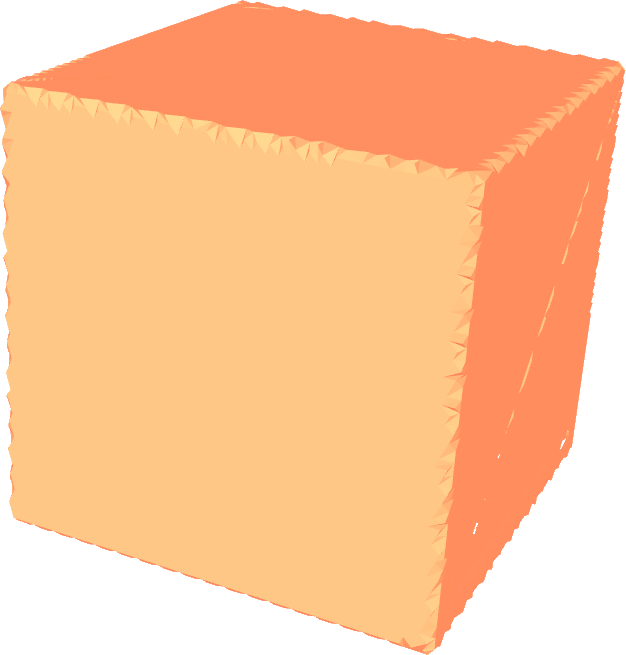
\includegraphics[width=.3\columnwidth]{figures/comparison/cube.png}
    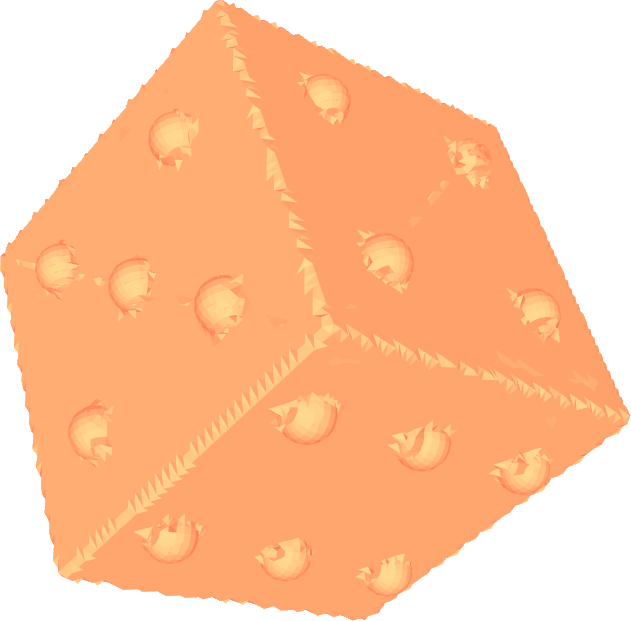
\includegraphics[width=.32\columnwidth]{figures/comparison/dice1.png}
    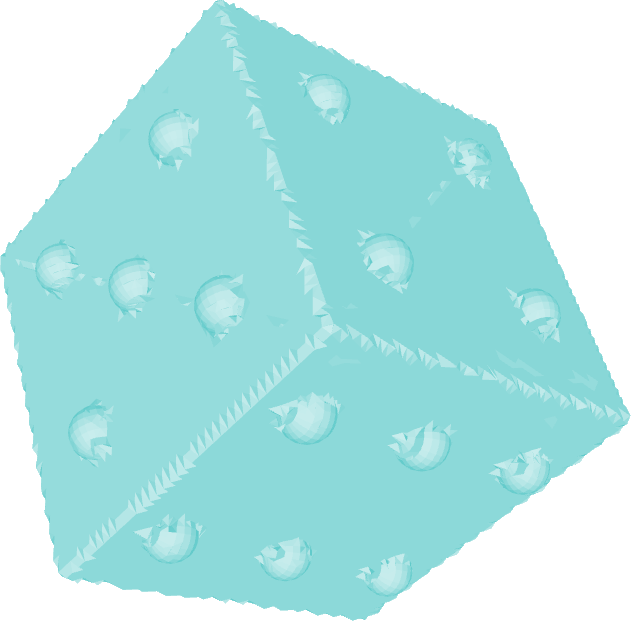
\includegraphics[width=.32\columnwidth]{figures/comparison/dice2.png}
    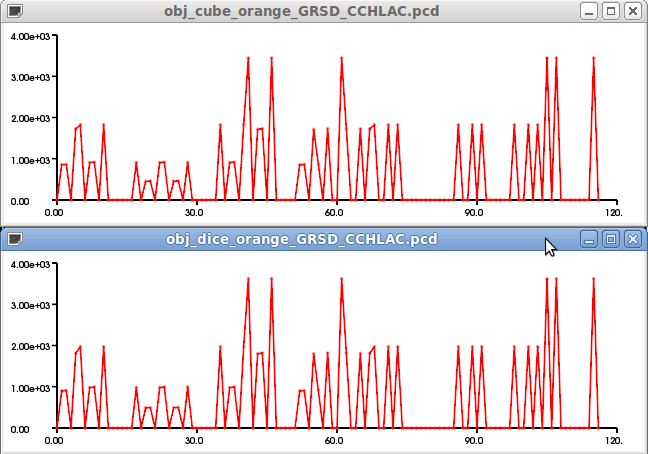
\includegraphics[width=.95\columnwidth]{figures/comparison/orange_cube_vs_orange_dice.png}
    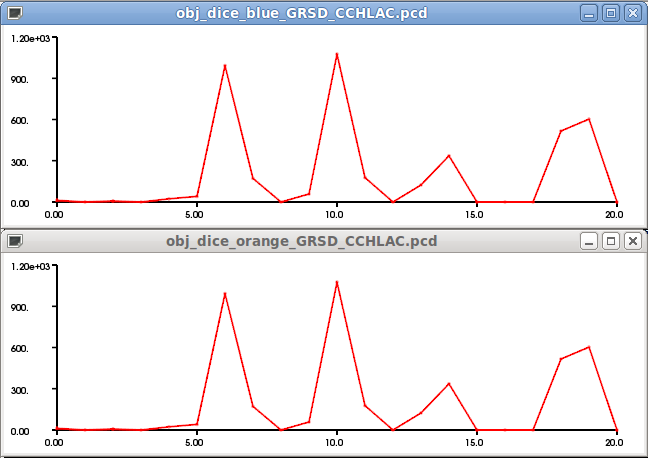
\includegraphics[width=.95\columnwidth]{figures/comparison/blue_vs_orange_dice_grsd.png}
  \caption{Color-CHLAC can not differentiate the dice from the cube (identical histograms in row 1 and 2), 
    while GRSD can not differentiate the different colors ((identical histograms in row 3 and 4)). 
    Their combination however produces different signatures for all of them (Figure~\ref{fig:grsd_cchlac}).}
  \label{fig:comparison}
\end{center}
\end{figure}

\section{Classification Methods}
\label{sec:classification}
\subsection{Linear Subspace Method}
\label{sec:subspace}
Linear Subspace Method (LSM)~\cite{watanabe1973} is an established learning method for classification. 
As a training process, several feature vectors that represent each object are extracted, 
and then Principal Component Analisis (PCA) for them is solved. 
Similarly to ~\cite{kanezaki2010icra}, we divide the whole voxel grid of each object into 
cubic subdivisions of a certain size, and then extract feature vectors from all the subdivisions for the training. 
Let the number of the subdivisions be $N$, the dimension of the feature vector be $d$, 
and the train feature vectors be $\bm{z}_t \in R^d, t=1,2,...N$. 
Then the eigenvectors of $R=\frac{1}{N} \sum^{N}_{t=1} \bm{z}_t \bm{z}_t^T$ are computed by solving the eigenvector problem. 
Note that we solve PCA for all the descriptors extracted from all the trained objects for the first step, 
and use top $d$ dimensions of the descriptor as a feature vector, in the same way as \cite{kanezaki2010icra}.

To classify and identify a detected object in environments, the system extracts one feature vector from the whole voxel grid of the object. 
Letting the feature vector be $\bm{z}$ and the matrix of top $r$ eigen vectors for the $i$-th object in the database be $P_i \equiv (\bm{v}_{i1} \bm{v}_{i2} ... \bm{v}_{ir})$,
the similarity between the query part and the $i$-th object in the database is calculated by the following equation:
\begin{eqnarray}\label{eq:y_calc}
  %\hspace{-1mm}
  y_i = \frac{\| P_i^T \bm{z} \|}{\| \bm{z} \|}
\end{eqnarray}

There is an advantage of using LSM with this kind of histogram-based descriptors which have additive property. 
The additive property means that a global descriptor for an object cluster equals the summation of local descriptors of its sub-parts. 
Owing to the property, one feature vector computed from each object cluster in environments can be classified by projecting it to 
   each subspace of database object, regardless of the size of the object cluster.

%\todo{Asako: Explain the advantage of additivity here.}
\subsection{Support Vector Machine-based Classification}
\todo{Zoli}

\section{Results}
\label{sec:results}
To evaluate VOSCH feature we ran \todo{WHICH ONE: cross-correlation?} tests 
using SVM and LSM classifiers on the two sets of data: 
i)set of 7 articially generated objects depicted in Figure~\ref{fig:grsd_cchlac}
with 7 different colors and ii)set of 63 objects of daily use scanned using
a Kinect device and a rotating table. We measured its recognition rate against
original implementations of ColorCHLAC and GRSD, and a simple concatentation
of histograms of both.
\subsection{Feature Extraction}
\label{sec:feature_extraction}
In all tests we parametrized the computation of the feature with the following parameters:
\begin{itemize}
\item search radius for normals: $2cm$
\item search radius for $r_{min}$ and $r_{max}$ estimation: $1cm$
\item voxel size: $1cm$
\end{itemize}

Following we performed the test on the computation times for the estimation
of VOSCH feature. The execution times are shown in the following table where $t1$
denotes the average estimation time per point, p an average number of points per object
and $t2$ denotes the average estimation time needed for 1 object:
\begin{table}[ht]
\begin{center}
\begin{tabular}{|c|c|c|c|}
\hline
 & $t1$ & $p$ & $t2$ \\
\hline
synthetic data (49 objects/49 views) & 36$\mu s$ & 19124 & 0.69s \\
\hline
real data (63 objects/1512 views) & 57$\mu s$ & 4632 & 0.26s \\
\hline
\end{tabular}
\caption{Time profile for the estimation of VOSCH feature}
\label{tbl:timing}
\end{center}
\end{table}
\subsection{Synthetic Data}

\todo{used 1 example of each object as training data and evaluated the model on 5 examples of each objects with 10 noise levels}

\todo{NOTE:} Since objects were uniformly colored and quite symmetrical, the fact that ColorCHLAC is not rotation invariant did not show up in the table.
In the original implementation ColorCHLAC was trained with artificial rotations to achieve rotation invariance.

\newcommand{\mc}[3]{\multicolumn{#1}{#2}{#3}}
\definecolor{tcA}{rgb}{0.784314,0.784314,0.784314}
\begin{table*}[ht]
\begin{center}
\begin{tabular}{|c|c|c|c|c|c|c|c|c|c|}\hline
% use packages: color,colortbl
\rowcolor{tcA} \textbf{} & \textbf{} & \mc{2}{>{\columncolor{tcA}}c|}{\textbf{GRSD (20D)}} & \mc{2}{>{\columncolor{tcA}}c|}{\textbf{Color-CHLAC (981D)}} & \mc{2}{>{\columncolor{tcA}}c|}{\textbf{Concatenated (1001D)}} & \mc{2}{>{\columncolor{tcA}}c|}{\textbf{VOSCH (137D)}}\\
\cline{3-10}
\rowcolor{tcA} \textbf{Noise STD} & \textbf{Rotation} & \textbf{LSM} & \textbf{SVM} & \textbf{LSM} & \textbf{SVM} & \textbf{LSM} & \textbf{SVM} & \textbf{LSM} & \textbf{SVM}\\
\hline
\mc{1}{|>{\columncolor{tcA}}c|}{\textbf{0.5}} & \mc{1}{>{\columncolor{tcA}}c|}{\textbf{None:}} & 14.2857\% & 14.2857\% & 100\% & 100\% & 100\% & 100\% & 100\% & 100\% \\
\rowcolor{tcA} \textbf{mm} & \textbf{Random:} & 14.2857\% & 12.6531\% & 36.3265\% & 70.2041\% & 78.7755\% & 79.5918\% & 100\% & 91.4286\% \\
\hline
\mc{1}{|>{\columncolor{tcA}}c|}{\textbf{1.0}} & \mc{1}{>{\columncolor{tcA}}c|}{\textbf{None:}} & 14.2857\% & 14.2857\% & 68.5714\% & 77.1429\% & 100\% & 85.7143\% & 100\% & 100\% \\
\rowcolor{tcA} \textbf{mm} & \textbf{Random:} & 14.2857\% & 14.2857\% & 30.6122\% & 65.7143\% & 78.3673\% & 78.7755\% & 100\% & 99.5918\% \\
\hline
\mc{1}{|>{\columncolor{tcA}}c|}{\textbf{1.5}} & \mc{1}{>{\columncolor{tcA}}c|}{\textbf{None:}} & 14.2857\% & 13.0612\% & 57.1428\% & 28.5714\% & 98.7755\% & 85.7143\% & 100\% & 91.4286\% \\
\rowcolor{tcA} \textbf{mm} & \textbf{Random:} & 14.2857\% & 13.0612\% & 25.7142\% & 26.1224\% & 72.6530\% & 82.449\% & 100\% & 90.6122\% \\
\hline
\mc{1}{|>{\columncolor{tcA}}c|}{\textbf{2.0}} & \mc{1}{>{\columncolor{tcA}}c|}{\textbf{None:}} & 14.2857\% & 12.2449\% & 39.1836\% & 28.5714\% & 85.7142\% & 85.7143\% & 100\% & 85.7143\% \\
\rowcolor{tcA} \textbf{mm} & \textbf{Random:} & 14.2857\% & 12.2449\% & 19.1836\% & 20.8163\% & 70.6122\% & 85.7143\% & 98.3673\% & 85.7143\% \\
\hline
\mc{1}{|>{\columncolor{tcA}}c|}{\textbf{2.5}} & \mc{1}{>{\columncolor{tcA}}c|}{\textbf{None:}} & 12.2448\% & 10.2041\% & 28.5714\% & 28.5714\% & 77.5510\% & 57.1429\% & 71.8367\% & 71.4286\% \\
\rowcolor{tcA} \textbf{mm} & \textbf{Random:} & 11.8367\% & 10.2041\% & 15.1020\% & 25.7143\% & 60.8163\% & 57.1429\% & 73.0612\% & 71.4286\% \\
\hline
\mc{1}{|>{\columncolor{tcA}}c|}{\textbf{3.0}} & \mc{1}{>{\columncolor{tcA}}c|}{\textbf{None:}} & 10.2040\% & 10.2041\% & 28.5714\% & 28.5714\% & 77.9591\% & 57.1429\% & 71.4285\% & 71.4286\% \\
\rowcolor{tcA} \textbf{mm} & \textbf{Random:} & 10.6122\% & 10.2041\% & 14.6938\% & 28.5714\% & 55.5102\% & 55.5102\% & 71.4285\% & 71.4286\% \\
\hline
\mc{1}{|>{\columncolor{tcA}}c|}{\textbf{3.5}} & \mc{1}{>{\columncolor{tcA}}c|}{\textbf{None:}} & 10.2040\% & 10.2041\% & 28.5714\% & 28.5714\% & 83.6734\% & 57.1429\% & 71.4285\% & 71.4286\% \\
\rowcolor{tcA} \textbf{mm} & \textbf{Random:} & 10.2040\% & 10.2041\% & 15.1020\% & 28.5714\% & 59.5918\% & 45.3061\% & 71.4285\% & 71.4286\% \\
\hline
\mc{1}{|>{\columncolor{tcA}}c|}{\textbf{4.0}} & \mc{1}{>{\columncolor{tcA}}c|}{\textbf{None:}} & 8.1632\% & 8.57143\% & 28.5714\% & 28.5714\% & 62.4489\% & 43.2653\% & 47.7551\% & 68.5714\% \\
\rowcolor{tcA} \textbf{mm} & \textbf{Random} & 7.3469\% & 8.57143\% & 18.7755\% & 28.5714\% & 57.1428\% & 42.8571\% & 52.2448\% & 70.2041\% \\
\hline
\mc{1}{|>{\columncolor{tcA}}c|}{\textbf{4.5}} & \mc{1}{>{\columncolor{tcA}}c|}{\textbf{None:}} & 6.5306\% & 8.16327\% & 14.2857\% & 28.5714\% & 57.1428\% & 42.8571\% & 42.8571\% & 74.2857\% \\
\rowcolor{tcA} \textbf{mm} & \textbf{Random:} & 6.9387\% & 7.7551\% & 18.3673\% & 28.5714\% & 48.1632\% & 44.898\% & 42.8571\% & 68.1633\% \\
\hline
\mc{1}{|>{\columncolor{tcA}}c|}{\textbf{5.0}} & \mc{1}{>{\columncolor{tcA}}c|}{\textbf{None:}} & 5.7142\% & 5.71429\% & 14.2857\% & 28.5714\% & 57.1428\% & 53.4694\% & 40.0000\% & 53.8776\% \\
\rowcolor{tcA} \textbf{mm} & \textbf{Random:} & 5.7142\% & 6.12245\% & 17.9591\% & 28.5714\% & 48.5714\% & 52.6531\% & 42.0408\% & 52.2449\% \\
\hline
\end{tabular}
\caption{Comparison of Features and Classifiers \todo{precision vs 1-recall for VOSCH?}}
\label{tbl:synthetic}
\end{center}
\end{table*}


\subsection{Real Data}
\subsubsection{Data Acquisition and Training}

Our database of 3D objects was obtained using the Kinect sensor.
The set of objects (see Figure~\ref{fig:robot}) encompasses the ones commonly used
in a typical household environment (mugs, utensils, books, etc) and is envisioned for a
larger expansion in the future.  In a pursue to account for a wide variety
of view angles, we rotated the objects on the rotating table with a given
angle-step ($15^\circ$ in the preliminary version) and acquired partial
snapshots from a human-eye perspective, i.e. the ones that the best
approximate the robot's view point during its working cycle.  We consider
this to be an important point as opposed to similar initiatives (e.g.,
\cite{kit}) where the datasets are acquired using high-precision but
non-affordable, fixed sensors, and thus not usable for applications such as ours.

\begin{figure}[htb!]
  \begin{center}
    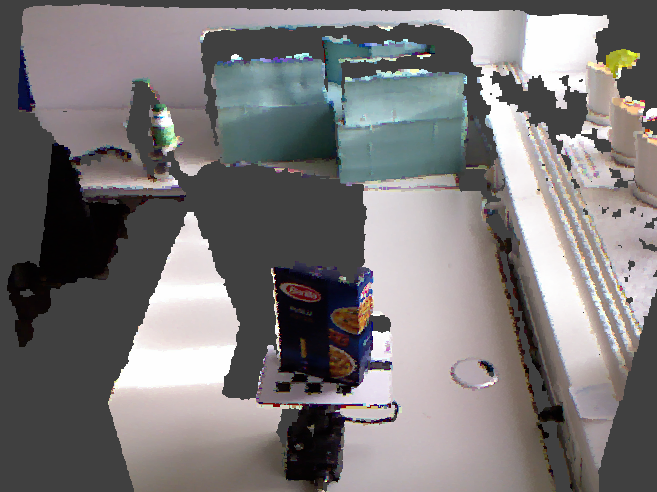
\includegraphics[width=.32\columnwidth]{figures/rot_table/barilla.png}
    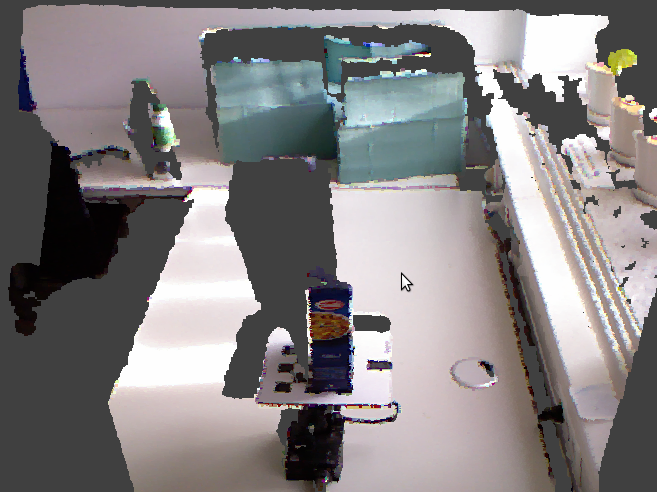
\includegraphics[width=.32\columnwidth]{figures/rot_table/barilla1.png}
    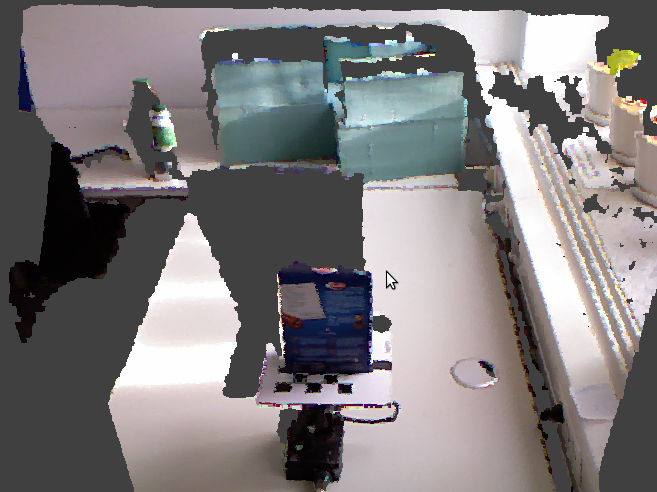
\includegraphics[width=.32\columnwidth]{figures/rot_table/barilla2.png}
    \caption{Acquisition of training data using a rotating table controlled by the robot.}
    \label{fig:data_acquisition}
  \end{center}
\end{figure}

\begin{figure}[htb!]
  \begin{center}
    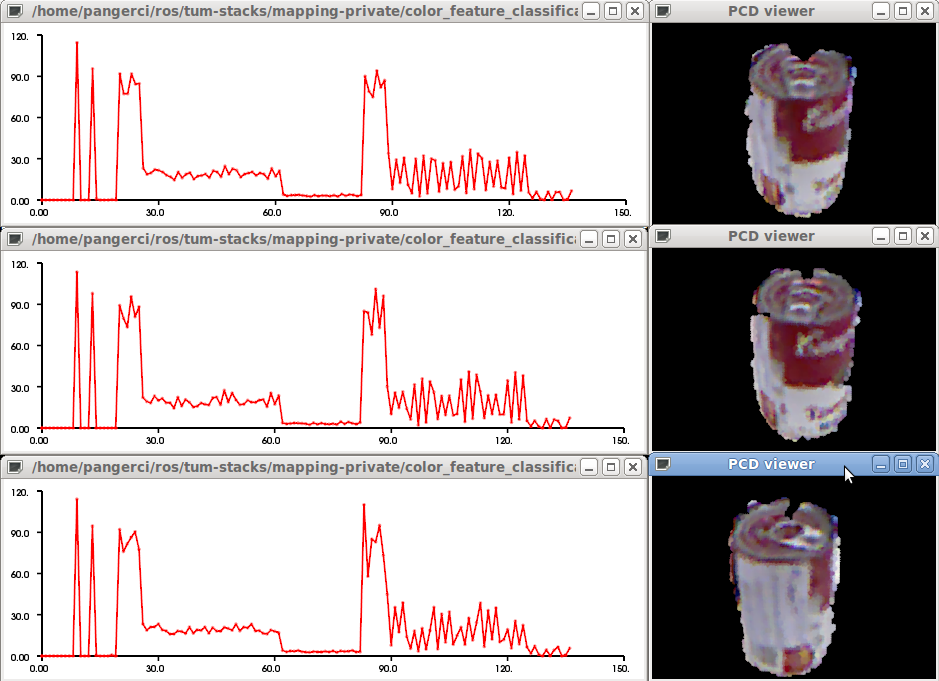
\includegraphics[width=.9\columnwidth]{figures/colorCHLAC/real/tomato/tomato_hist_pcd.png}
    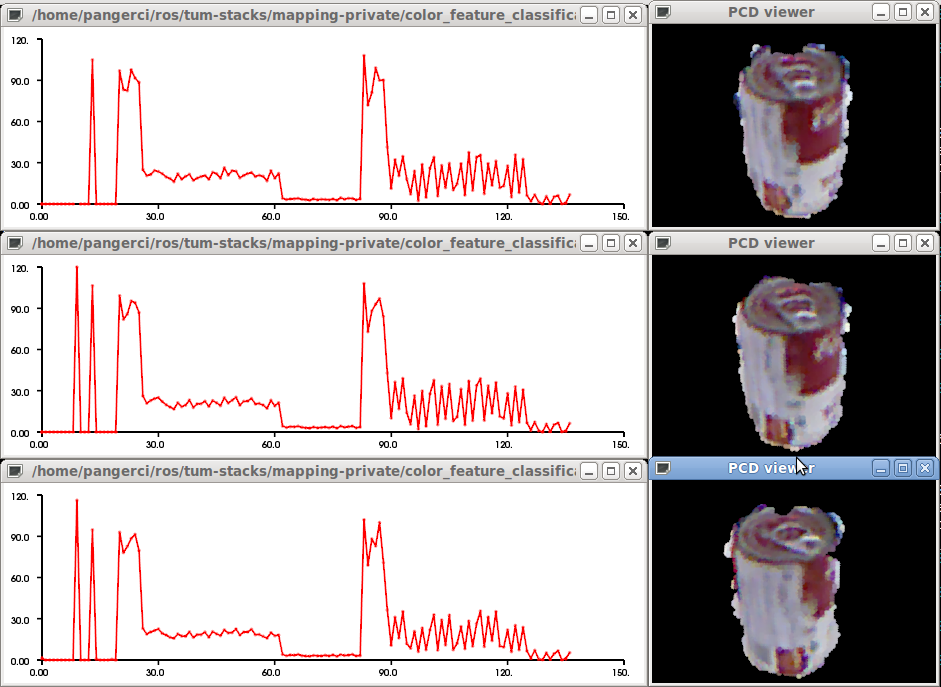
\includegraphics[width=.9\columnwidth]{figures/colorCHLAC/real/tomato/tomato_hist_pcd2.png}
    \caption{Examples of \todo{scaled} VOSCH histograms for a Tomato Soup can.}
    \label{fig:grsd_colorchlac_tomato}
  \end{center}
\end{figure}


\subsubsection{Evaluation on Training Data}

\todo{ALL: split training data into 2 groups and evaluate classification of one using the model computed for the other. Or complete cross-correlation.}

\begin{table*}[ht]
\begin{center}
\begin{tabular}{|c|c|c|c|c|}
\hline
\rowcolor{tcA} & \textbf{GRSD (20D)} & \textbf{Color-CHLAC (981D)} & \textbf{Concatenated (1001D)} & \textbf{VOSCH (137D)} \\
\hline
\mc{1}{|>{\columncolor{tcA}}c|}{\textbf{LSM}} & 29.6958\% (17.2619\%) & 99.0741\% (97.8175\%) & 99.3386\% (96.8915\%) & 97.8836\% (93.1217\%) \\
\hline
\mc{1}{|>{\columncolor{tcA}}c|}{\textbf{SVM}} & 99.2063\% (66.9974\%) & 99.8677\% (99.6693\%)  & 99.9339\% (99.6032\%) & 100\% (99.1402\%) \\
\hline
\end{tabular}
\caption{Model Accuracy on Real Training Data (and Leave-One-Out Test) for VOSCH \todo{less decimals and 1 column}}
\label{tbl:training}
\end{center}
\end{table*}

Table~\ref{tbl:training} shows the percentage of correctly classified training examples using the model computed for them,
and the percentage of correctly classified views using the model constructed using the remaining views.

\subsubsection{Evaluation on Novel Views}

\todo{Prove it works for a)textured objects, b)texture-less objects, c)objects with different shapes, 
d)varying lighting conditions -- no clutter, 1 object at a time}
%\todo{Dejan}

\subsection{Object Detection Pipeline (in Clutter)}
\label{sec:recognition}
\todo{Asako: Reduce the amount of the texts here.}
We applied our object recognition method on an object detection scheme in a cluttered environment.
The system computes the similarities between each target object and all rectangular-solid sub-regions in the environment, and then it outputs all the regions that have higher similarities than a certain threshold as the candidates of the target object.
Each sub-region has the same size as that of the bounding box of the target object.
To accelerate feature extraction from the sub-regions, we used ``Integral Feature Table''~\cite{kanezaki2010tvc}, which is a simple extension of ``Integral Image''~\cite{viola2001} from 2D to 3D.
The ``Integral Feature Table'' $\bm{I}(x,y,z)$ is defined as the $d$-dimensional compressed feature vector extracted from the voxel area
    ranging from $(0,0,0)$ to $(x,y,z)$.
Let the feature vector of the voxel area with $x$ ranging from $x_1$ to $x_2$,
    $y$ ranging from $y_1$ to $y_2$, and $z$ ranging from $z_1$ to $z_2$, be $\bm{F}(x_1,y_1,z_1,x_2,y_2,z_2)$.
This is computed by the following equation:
\begin{eqnarray*}\label{eq:sat}
\bm{F}(x_1,y_1,z_1,x_2,y_2,z_2) = \bm{I}(x_2,y_2,z_2) - \bm{I}(x_1,y_2,z_2)
                           \\ - \bm{I}(x_2,y_1,z_2) - \bm{I}(x_2,y_2,z_1)
                           \\ + \bm{I}(x_1,y_1,z_2) + \bm{I}(x_1,y_2,z_1)
                           \\ + \bm{I}(x_2,y_1,z_1) - \bm{I}(x_1,y_1,z_1)
\end{eqnarray*}
Using the ``Integral Feature Table'', $\bm{F}(x_1,y_1,z_1,x_2,y_2,z_2)$ can always be computed by adding the 8 cached feature vectors,
    regardless of the size of the target object.
Note that this is not effective when the number of sub-regions included in the detection box is smaller than 8.
Within the large color voxel data of an environment,
   only the voxels on the surface of each object have RGB values, while other voxels have the empty property.
This means that the object detection process can be accelerated by skipping empty regions.
Similarly to the ``Integral Feature Table'', we create a table that stores
   the number of voxels with the occupied property, in the area ranging from $(0,0,0)$ to $(x,y,z)$.
Using this table, the number of voxels with the occupied property in the detection box can be computed quickly by adding 8 scalar values.
If the number is less than a certain threshold $h$,
   the system skips the similarity calculation and moves the detection box forwards.
In this work, we set $h$ to the minimum value of the occupied voxel number in the training samples of the target object.

\todo{Asako: description for the results}


% \begin{figure}[htb!]
%   \begin{center}
%     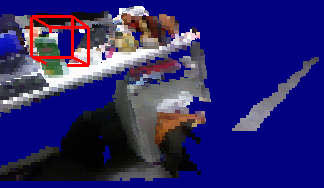
\includegraphics[width=.45\columnwidth]{figures/colorCHLAC/detection7.png}
%     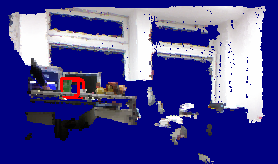
\includegraphics[width=.45\columnwidth]{figures/colorCHLAC/detection5.png} \\
%     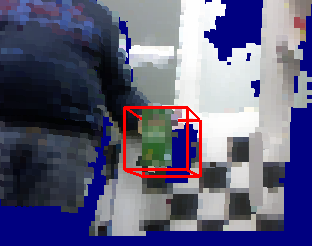
\includegraphics[width=.9\columnwidth]{figures/colorCHLAC/detection2.png}
%     \caption{An example of the detection of tetrahedral package of milk.}
%     \label{fig:milk_testing}
%   \end{center}
% \end{figure}


\section{Conclusions and Future Work}
\label{sec:conclusion}
\todo{ALL}
\begin{itemize}
\item automatic in-hand building of models
\item color stabilization
\item new geometric part - Zoli
\end{itemize}

% \section*{Acknowledgments}
% This work was supported by the DFG cluster of excellence \emph{CoTeSys} (Cognition for Technical Systems).\\
% \todo{Asako: Do we need to ackknowledge someone from ISI Lab?}
% %% Use plainnat to work nicely with natbib.

\bibliographystyle{plainnat}
\bibliography{references}

\end{document}


%TODO:
%Check the original template and see what the meant with the hyperlinks
%GRSD: 20 or 21 dimensions
